\documentclass{beamer}
\usepackage{tikz}
\usetikzlibrary{calc}
\usetikzlibrary{arrows.meta}
\usetikzlibrary{backgrounds,matrix,fadings,calc,positioning,decorations.pathreplacing,decorations.markings,arrows.meta,shapes,shapes.multipart}
\usetikzlibrary{patterns,math,quotes,positioning,angles}
\usetikzlibrary{spy}
\usepackage{pgfplots}
\usepackage{xcolor}
\usepackage{chemfig}
\usepackage{amsmath}
\usepackage{subfiles}
\usepackage{shellesc}
% Fur Makros mit Key-Value-Pairs
\usepackage{keycommand}
\usepackage[mode=buildnew]{standalone}% requires -shell-escape
\usepackage[decimalsymbol=comma, per-mode=fraction]{siunitx}
\usepgfplotslibrary{fillbetween}
\usetikzlibrary{external}
\tikzexternalize[prefix=tikzpictures/]
\usepackage[version=4]{mhchem}

\usetheme{Berlin}
\usecolortheme{default}

\title[Condensation and Evaporation of Hexane in Nanoporous Alumina Membranes]{Condensation and Evaporation of Hexane in Nanoporous Alumina Membranes}
%\subtitle{}
\author[Hermann Böttcher]{Hermann Böttcher\inst{1} \and Victor Doebele\inst{2} \and Pierre-Etienne Wolf\inst{2} \and Panayotis Sphatis\inst{2} \and Fabien Souris\inst{2}}
\institute{
          \inst{1}University of Constance
          \and
          \inst{2}Institut Néel, Centre national de la recherche scientifique
          }
\date[Constance, 02/10/2018]{02/10/2018}
%\logo{
\includegraphics[height=1.5cm]{graphics/logoNEEL.png}}

\begin{document}

  \frame{\maketitle}

  %\subfile{slides/slide_1.tex}
  %\subfile{slides/slide_2.tex}
  %\subfile{slides/slide_3.tex}
  %\subfile{slides/slide_4.tex}
  %\subfile{slides/slide_5.tex}
  %\subfile{slides/slide_6.tex}
  %\subfile{slides/slide_7.tex}
  %\subfile{slides/slide_8.tex}
  %\subfile{slides/slide_9.tex}
  %\subfile{slides/slide_10.tex}
  %\subfile{slides/slide_11.tex}
  %\subfile{slides/slide_12.tex}
  %\subfile{slides/slide_13.tex}
  %\subfile{slides/slide_14.tex}
  %\subfile{slides/slide_15.tex}
  \subfile{slides/slide_16.tex}
  \subfile{slides/slide_17.tex}
  %\subfile{slides/slide_18.tex}


  \begin{frame}{Inverse funnelling}

  \end{frame}



  \begin{frame}{Atomic layer deposition}

  \end{frame}



%  \begin{frame}{SEM image analysis}
%    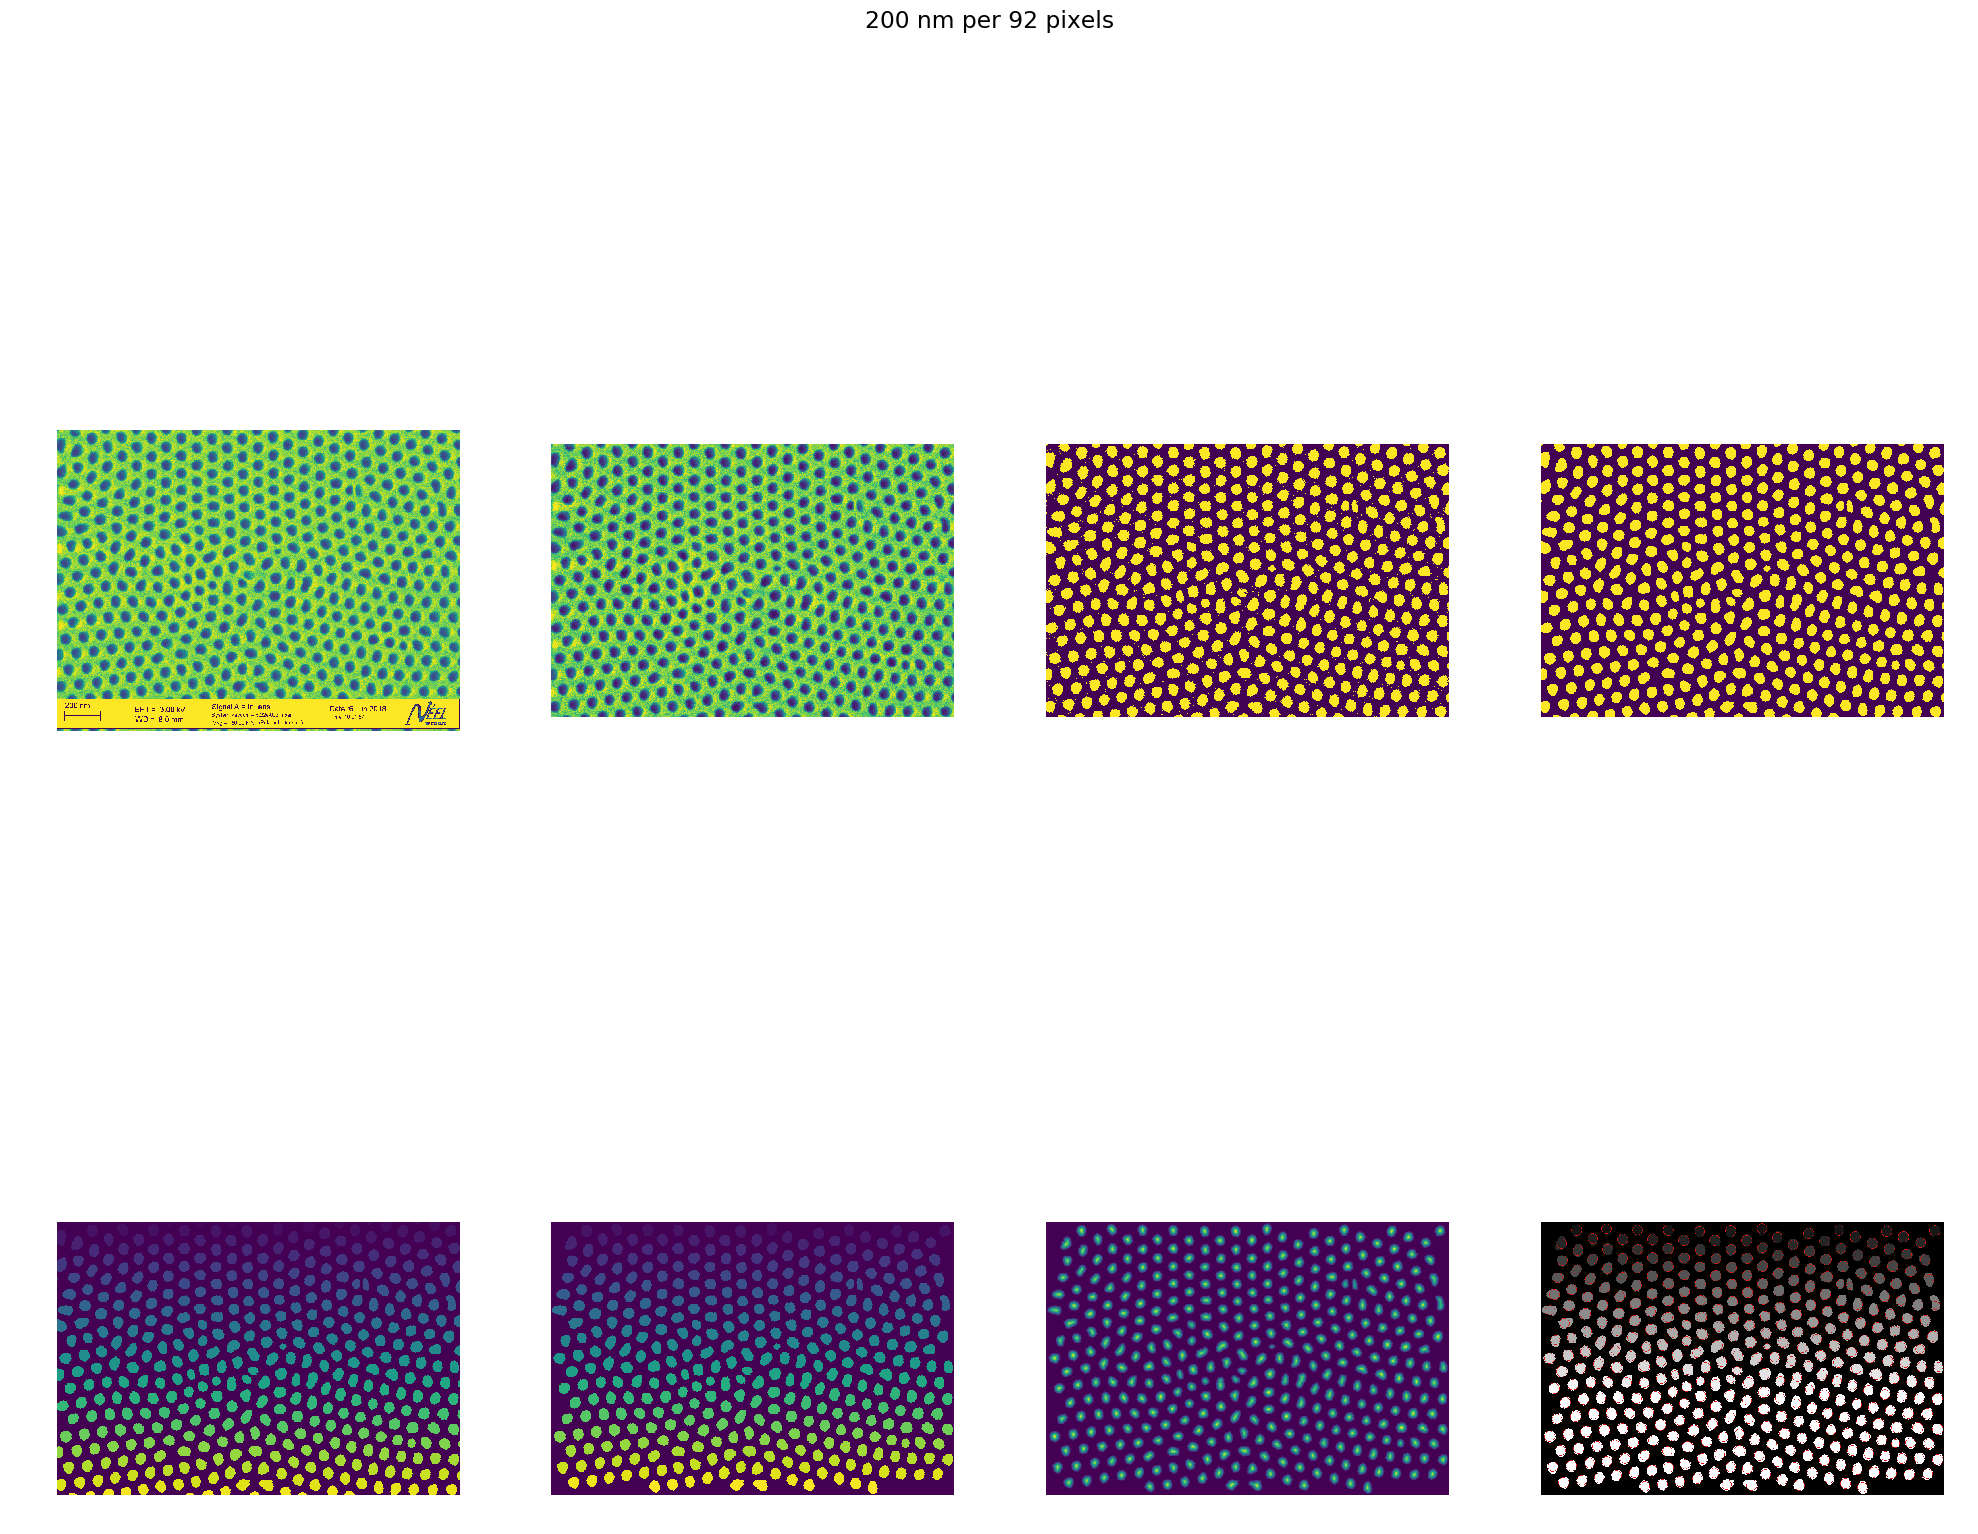
\includegraphics[width=\linewidth]{images/AAM_295_PO_30 um_Al_26.png}
%  \end{frame}


\end{document}
